\section{Auswertung}
\label{sec:Auswertung}

% Radius kl. Kugel: 0.7785 und Durchmesser kl. Kugel: 1.557 (in cm)
% Radius gr. Kugel: 0.788 und Durchmesser gr. Kugel: 1.576 (in cm)
% Dichte kl. Kugel: 2.253191 (in g/cm^3) oder 2253.190896 (in kg/m^3)
% Dichte gr. Kugel: 2.416482 (in g/cm^3) oder 2416.481804 (in kg/m^3)
% Gemittelte Fallzeit (hoch) kl: 12.203, gr: 34.751999999999995
% Gemittelte Fallzeit (runter) kl: 12.142000000000001, gr: 34.727999999999994
% eta_hoch(Viskosität): 1.1700331290528003 (in mPa*s)
% eta_runter(Viskosität): 1.1641844016192004 (in mPa*s)
% Apparatekonstante K_gr_h: 0.023738753324280895 (in mPa*cm^3/g)
% Apparatekostante K_gr_r: 0.02363641222658268 (in mPa*cm^3/g)
% Reynoldschezahl Re_kl_h: 55.0911779489854
% Reynoldschezahl Re_kl_r: 55.64611179702035
% Reynoldschezahl Re_gr_h: 9.672502942441714
% Reynoldschezahl Re_gr_r: 9.727814579581626
% K_kl = 0.07640 # in m*Pa*cm^3/g (gegeben)
% dichte_wasser = 0.998207 # in g/cm^3 (Internet)

\begin{figure}
  \centering
  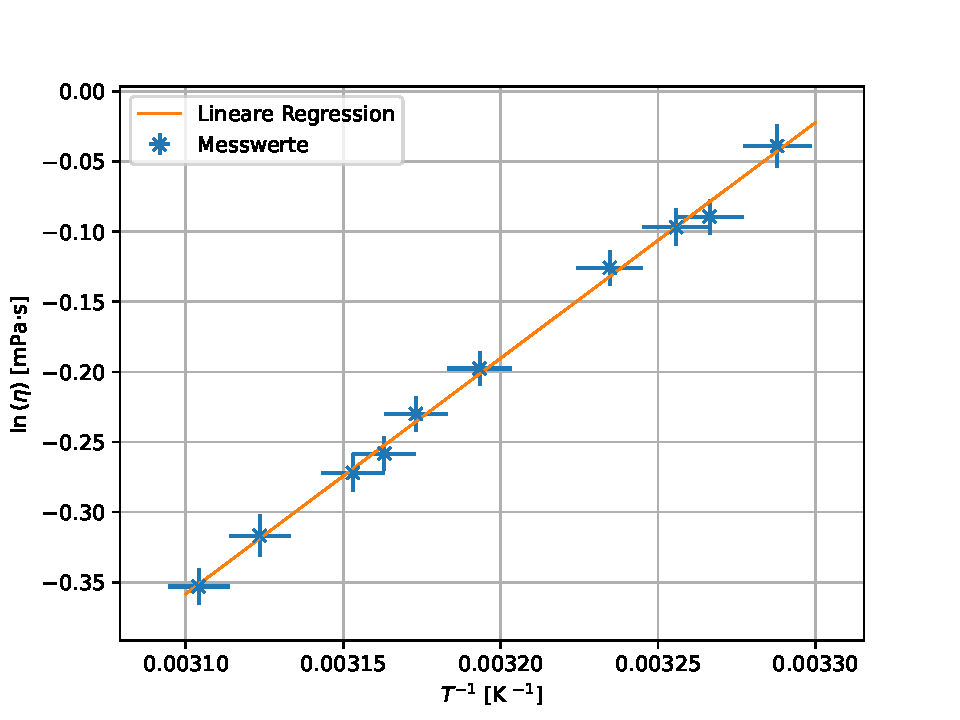
\includegraphics{plot.pdf}
  \caption{Plot.}
  \label{fig:plot}
\end{figure}

%Siehe \autoref{fig:plot}!